\newpage
\genHeader
\hypertarget{validate common}{} 
\section{Validate your installation with JUnit}

\begin{itemize}

\item[$\blacktriangleright$] In Eclipse, choose \texttt{Working Sets} as your top level element in the package explorer (Fig.~\ref{eclipse:topLevel}), as we use
them to structure the workspace.

\begin{figure}[htbp]
	\centering
  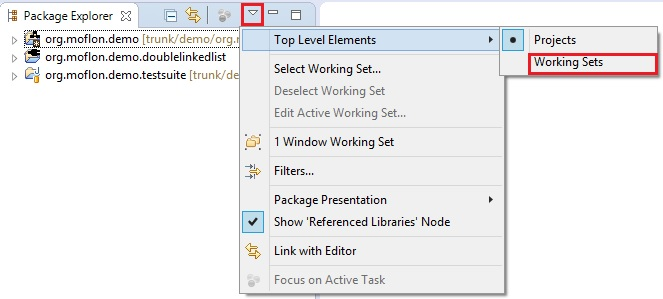
\includegraphics[width=0.9\textwidth]{eclipse_explorerWorkingsets}
	\caption{Top level elements in Eclipse}
	\label{eclipse:topLevel}
\end{figure}

\item[$\blacktriangleright$] Locate ``Other Projects/DemoTestSuite.'' This is the testsuite imported with the demo files to make sure everything has been installed and
set up correctly. Right click on the project to bring up the context menu and go to ``Run As/JUnit Test.'' If anything goes wrong, try refreshing by choosing
your metamodel project and pressing  \texttt{F5}, or right-clicking and selecting \texttt{Refresh}.

\vspace{0.5cm}

\begin{figure}[htbp]
	\centering
  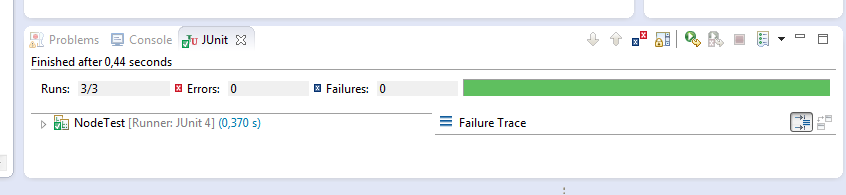
\includegraphics[width=1\textwidth]{eclipse_passedJUnitTest}
	\caption{All's well that ends well\ldots}
	\label{eclipse:passedTest}
\end{figure}

\vspace{0.5cm}

Congratulations!  If you see a green bar  (Fig.~\ref{eclipse:passedTest}), then everything has been set up correctly and you are now ready to start
metamodelling!

\jumpDual{projectStructure vis}{projectStructure tex}

\end{itemize}